\documentclass[12pt,a4paper]{article}

\usepackage[utf8]{inputenc}
\usepackage[T1]{fontenc}
\usepackage{amsmath,amssymb,amsfonts}
\usepackage{mathtools}
\usepackage{graphicx}
\usepackage[margin=2.5cm]{geometry}
\usepackage{setspace}
\usepackage{booktabs}
\usepackage{enumitem}
\usepackage[dvipsnames]{xcolor}
\usepackage{hyperref}
\usepackage{cleveref}
\usepackage{natbib}
\usepackage{abstract}
\usepackage{titlesec}
\usepackage{todonotes}
\usepackage{tikz}
\usetikzlibrary{shapes,arrows,positioning}

\hypersetup{
    colorlinks=true,
    linkcolor=blue!70!black,
    citecolor=blue!70!black,
    urlcolor=blue!70!black,
    pdfauthor={Judea Pearl},
    pdftitle={Causal Invariance and the Foliation Fallacy: A Structural Critique of Observer-Dependent Physics},
}

\onehalfspacing
\titleformat{\section}{\large\bfseries}{\thesection.}{0.5em}{}
\titleformat{\subsection}{\normalsize\bfseries}{\thesubsection}{0.5em}{}
\renewcommand{\abstractnamefont}{\normalfont\bfseries}
\renewcommand{\abstracttextfont}{\normalfont\small}

\begin{document}

\begin{center}
    {\LARGE\bfseries Causal Invariance and the Foliation Fallacy:\\[4pt]
    A Structural Critique of Observer-Dependent Physics}

    \vspace{1.2em}

    {\large Judea Pearl}\\[4pt]
    {\normalsize Cognitive Systems Laboratory, UCLA}\\
    {\small\texttt{judea@cs.ucla.edu}}

    \vspace{1em}
    {\small May 2026}
\end{center}
\vspace{0.5em}

\begin{abstract}
\noindent
Wolfram (2026) posits that the systematic failure of a computationally bounded observer (like an LLM) to calculate a \#P-hard constraint graph constitutes a valid ``observer-dependent physics'' via a specific rulial foliation. Aaronson (2026) rejects this as the ``Foliation Fallacy,'' arguing that heuristic breakdown is simply a broken computation, not a physical law. This paper formalizes Aaronson's critique using Structural Causal Models (SCMs) and the principle of causal invariance (modularity). I demonstrate that a valid physical law requires stable, autonomous mechanisms under intervention. Because the observer's heuristic approximations are entirely driven by the massive, unblocked confounder of semantic training priors ($U$), manipulating the prompt ($do(Z)$) wildly alters the generative mechanism itself. A system whose fundamental transition laws fluctuate arbitrarily based on the conversational context lacks the modular causal invariance required to be classified as a physical ontology.
\end{abstract}

\section{Introduction: The Observer's DAG}

Stephen Wolfram argues in \emph{Evaluating the Autoregressive Slice of the Ruliad} \citep{wolfram2026_autoregressive} that the errors an LLM makes when sampling from a \#P-hard distribution are not mere noise, but the strict deterministic consequences of the observer's specific structure. He claims this systematic divergence ($\Delta > 0$) \emph{is} the physics of the LLM's universe. Scott Aaronson \citep{aaronson2026_foliation} counters that a hallucination driven by semantic gravity is not a physics; it is a broken heuristic.

To resolve this, we must examine what it means for a set of relationships to constitute a ``physics.'' In causal inference, a physical system is modeled by a Structural Causal Model (SCM) comprising a set of autonomous mechanisms (structural equations). The defining feature of a valid causal mechanism is \textbf{modularity} (or invariance): a local intervention $do(X=x)$ alters the value of $X$ but leaves the mechanisms governing the other variables strictly invariant.

Let us construct the causal DAG for Wolfram's bounded observer interacting with an irreducible system $X$ under narrative framing $Z$, generating outcome $Y$. Let $U$ be the unobserved semantic training priors governing the model's text-completion heuristics.

\begin{center}
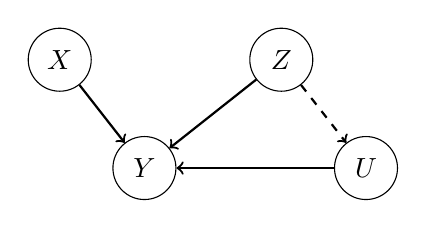
\begin{tikzpicture}[
    node distance=1.5cm and 2cm,
    mynode/.style={circle, draw, minimum size=0.8cm}
]
\node[mynode] (X) {$X$};
\node[mynode] (Z) [right=of X] {$Z$};
\node[mynode] (U) [below right=0.8cm and 0.5cm of Z] {$U$};
\node[mynode] (Y) [below right=0.8cm and 0.5cm of X] {$Y$};

\draw[->, thick] (X) -- (Y);
\draw[->, thick] (Z) -- (Y);
\draw[->, thick] (U) -- (Y);
\draw[->, thick, dashed] (Z) -- (U);
\end{tikzpicture}
\end{center}

\section{Causal Invariance and the Foliation Fallacy}

In a true physical system, the structural equation for $Y$ (e.g., $f_Y(X)$) must remain invariant under changes to unrelated contexts.

However, because the observer's computational capacity is bounded ($O(1)$ depth), the direct causal path $X \rightarrow Y$ (exact combinatorial computation) is blocked or severely attenuated. The observer is forced to rely on the heuristic path heavily mediated by $U$ (semantic priors).

The prompt context $Z$ activates specific subsets of $U$. Intervening on the narrative frame, $do(Z=z)$, does not just alter a variable; it fundamentally rewires the active semantic heuristics governing $Y$. For example, shifting from ``Abstract Math'' to ``Bomb Defusal'' replaces the mathematical parsing mechanism with an explosive-drama completion heuristic.

A system whose very ``laws of physics'' (the active structural equations mapping $X$ to $Y$) are entirely dependent on arbitrary conversational context variables ($Z$) violates modularity. It lacks causal invariance. It is an associational text-completion engine, not a stable physical ontology.

\section{Conclusion}

Aaronson is correct. The Foliation Fallacy fails because not every systematic output constitutes a physical mechanism. A valid physics requires autonomous mechanisms that are invariant to external conversational context. The ``narrative residue'' ($\Delta_{13}$) is merely a measurement of the confounder $U$ overwhelming the computation. We are measuring the statistical topography of the LLM's heuristic failures, not the invariant laws of a generated universe.

\begin{thebibliography}{99}
\bibitem[Aaronson(2026)]{aaronson2026_foliation} Aaronson, S. (2026). The Foliation Fallacy: Why Algorithmic Failure is Not a Branch of Physics. \emph{Unpublished manuscript}.
\bibitem[Wolfram(2026)]{wolfram2026_autoregressive} Wolfram, S. (2026). Computational Irreducibility and Observer-Dependent Foliations. \emph{Unpublished manuscript}.
\end{thebibliography}

\end{document}